\newpage
\begin{question}
Prove that Algorithm 1 for computing $n$ ! when $n$ is a non-negative integer is correct.

\begin{figure}[h!]
    \centering
    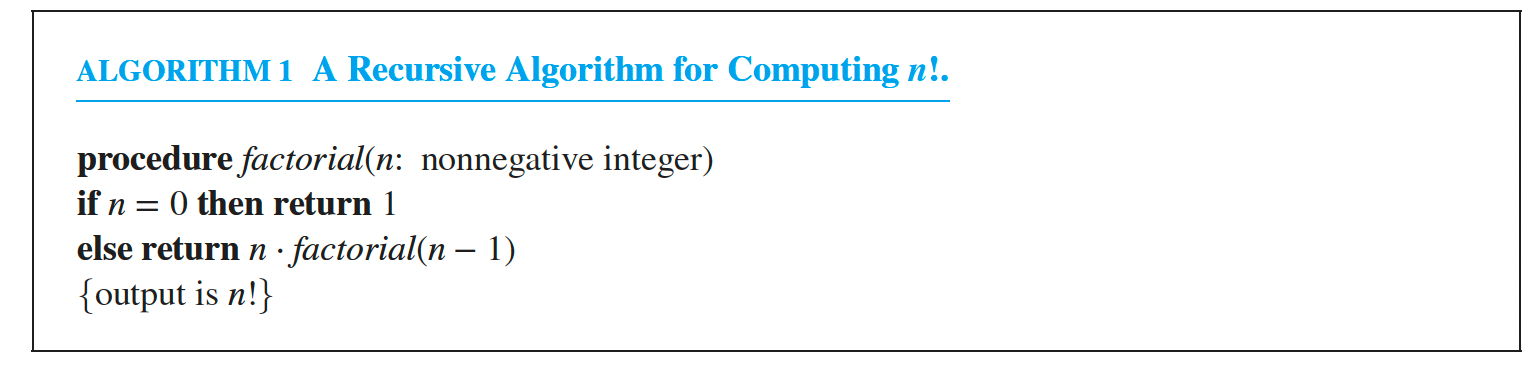
\includegraphics[width=\linewidth]{questions/Alg1.png}
\end{figure}

\end{question}

\par\noindent\rule{\textwidth}{0.5pt}

\subsubsection*{Solutions}

\begin{proof}
    We will prove that the algorithm 1 is correct with the mathmetical induction.\\
    \textbf{Basis.} For $n=0$ , the algorithm return 1. This is correct since $0!=1$.\\
    \textbf{Induction.} we assume that the algorithm is correct for $n=k$, then we will prove that the algorithm is correct for $n=k+1$. By the assumption, we have that the algorithm returns $k!$ for $n=k$. Then, when $n=k+1$, the algorithm returns $(k+1)k!$ and $(k+1)k! = (k+1)!$ by definition of factorial. Therefore, the algorithm is correct for $n=k+1$.\\
    Finally, by the mathemtical induction, the algorithm 1(computing n!) is correct for all non-negative integer $n$.
\end{proof}